%----------------------------------------------------------------------------------------
%	METODE
%----------------------------------------------------------------------------------------
\section*{HASIL DAN PEMBAHASAN}

\subsection*{Analisis}
Pada penelitian ini, akan dibangun sebuah perangkat lunak untuk membangkitkan kemungkinan jalur dari sebuah program. Jalur-jalur ini dapat dijadikan dasar untuk membangkitkan data uji agar data uji yang digunakan untuk pengujian dapat mewakili semua kemungkinan. Untuk memonitor jalur mana yang dilalui ketika diberikan masukan data uji, maka sistem ini juga akan melakukan penyisipan tag-tag sebagai instrumentasi ke dalam kode program secara otomatis.

Sebelumnya sudah terdapat beberapa program yang dapat membangkitkan CFG seperti Eclipse  Control Flow Graph Generator tetapi \textit{library} tersebut hanya dapat digunakan di eclipse dan hanya membangkitkan CFG dari kode program java. 

Data yang digunakan dalam penelitian ini didapatkan dari penelitian yang dilakukan oleh \citeauthor{HERMADI2015} (\cite*{HERMADI2015}). Terdapat 15 contoh program yang akan digunakan pada penelitian ini dengan tingkat kompleksitas yang beragam. Contoh program yang akan digunakan dapat dilihat pada \ref{tab:jadwal}.
 
 \begin{table*}[h!]
 	\begin{center}
 		\caption{Contoh program uji}
 		\label{tab:jadwal}
 		\footnotesize
 			\begin{tabular}{|l|l|l|p{9cm}|}
 				\hline
 				\rowcolor[HTML]{EFEFEF} 
 				\multicolumn{1}{|c|}{\cellcolor[HTML]{EFEFEF}\textbf{No}} & \multicolumn{1}{c|}{\cellcolor[HTML]{EFEFEF}\textbf{\begin{tabular}[c]{@{}c@{}}Program\\   Uji\end{tabular}}} & \multicolumn{1}{c|}{\cellcolor[HTML]{EFEFEF}\textbf{Nama}} & \multicolumn{1}{c|}{\cellcolor[HTML]{EFEFEF}\textbf{Deskripsi}}                                                       \\ \hline
 				1                                                         & triangleAhmed2008                                                                                             & tA2008                                                     & Menentukan tipe dari segitiga apakah termasuk equilateral, isosceles, scalene, atau not triangle                      \\ \hline
 				2                                                         & minimaxiAhmed2008                                                                                             & mmA2008                                                    & Menentukannilai minimal dan maksimal dari inputan berupa bilangan  dalam array                                        \\ \hline
 				3                                                         & insertionAhmed2008                                                                                            & iA2008                                                     & Mengurutkan bilangan dalam array menggunakan metode insertion sort                                                    \\ \hline
 				4                                                         & binnaryAhmed2008                                                                                              & binA2008                                                   & mencari indeks sebuah bilangan dalam array dengan mengembalikan indeks jika ditemukan dan tidak jika tidak ditemukan. \\ \hline
 				5                                                         & bubbleAhmed2008                                                                                               & bubA2008                                                   & Mengurutkan bilangan dalam array menggunakan metode bubble sort                                                       \\ \hline
 				6                                                         & gcdAhmed2008                                                                                                  & gA2008                                                     & Menghitung GCD atau pembagi dua bilangan terbesar                                                                     \\ \hline
 				7                                                         & expintBueno2002                                                                                               & eB2002                                                     & Fungsi exponensial yang dapat memproses bilangan integer dan float                                                    \\ \hline
 				8                                                         & quotientBueno2002                                                                                             & qB2002                                                     & Menghitung hasil bagi dan sisa hasil bagi dari dua buah bilangan bulat positif                                        \\ \hline
 				9                                                         & findBueno2002                                                                                                 & fB2002                                                     & Mengurutkan bilangan dalam array sebagian                                                                             \\ \hline
 				10                                                        & fitnessMiniMaxiHermadi2014                                                                                    & fmH2014                                                    & Menghitung fungsi fitness dari fungsi minimaxiAhmed2008                                                               \\ \hline
 			\end{tabular}
 		\normalsize
 	\end{center}
 \end{table*}

\subsection*{Perancangan}

\subsubsection*{Perancangan \textit{Class Diagram}}
Class diagram dibangun untuk menggambarkan struktur sistem dari segi pendefinisian class-class. Perancangan Class diagram dapat dilihat pada Gambar \ref{fig:classdiagram}.
\begin{figure}[h!]
	\centering
	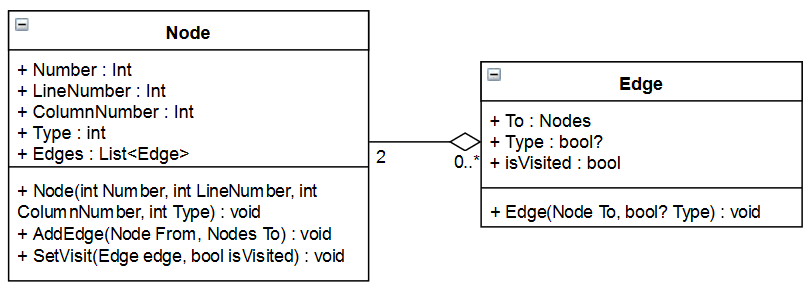
\includegraphics[width=230pt]{gambar/classdiagram}
	\caption{\textit{Perancangan \textit{Class Diagram}}}
	\label{fig:classdiagram}
\end{figure}
\textit{Class graph} memiliki atribut berupa list dari class node. Dalam sebuah \textit{class node} terdapat informasi nomor \textit{node}, nomor baris dan kolom dari kode program, tipe dari perintah tersebut. Selain itu, terdapat list edge yang berisi \textit{node} tujuan dan tipe dari \textit{edge} yang digunakan jika terdapat percabangan apakah \textit{true}, \textit{false}, atau hanya garis penghubung biasa.
\subsubsection*{Perancangan Antarmuka}
Perancangan antarmuka meliputi perancangan antarmuka form untuk pengguna memasukkan kode program yang akan di proses dan antarmuka hasil dari proses yang telah dilakukan. Perancangan antarmuka hasil dari proses yang telah dilakukan dapat dilihat pada Gambar \ref{fig:perancanganantarmuka}.
\begin{figure}[h!]
	\centering
	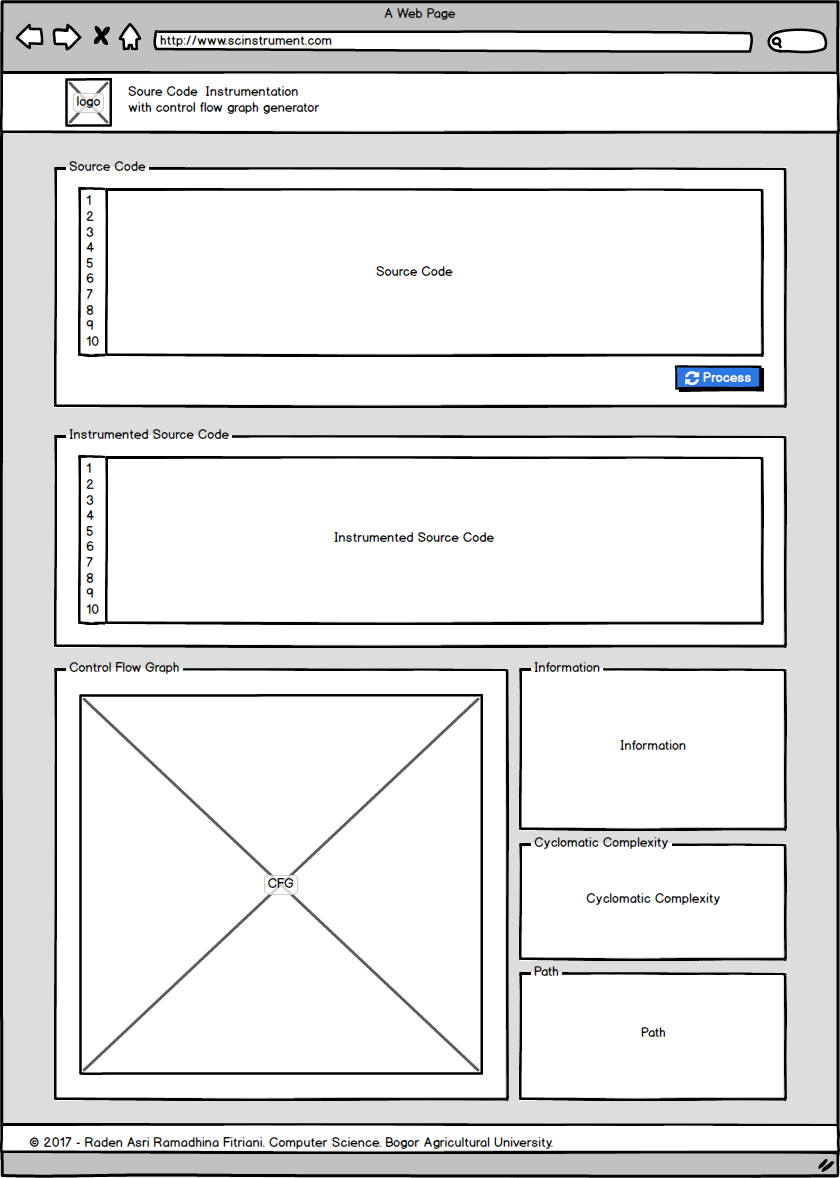
\includegraphics[width=230pt]{gambar/perancanganantarmuka}
	\caption{\textit{Perancangan antarmuka sistem}}
	\label{fig:perancanganantarmuka}
\end{figure}

\subsection*{Implementasi}

Aplikasi dibangun dengan menggunakan bahasa pemrograman C\# dan menggunakan IDE Microsoft Visual Studio Ultimate 2013. 

Sebagai contoh, kode program yang digunakan adalah tA2008. Pada kode tA2008 terdapat perintah IF-THEN-ELSE bersarang sebanyak tiga tingkat. 

\subsubsection*{Kode Program}
Gambar \ref{fig:tA2008} merupakan kode program tA2008, yaitu fungsi untuk mencari jenis dari segitiga jika diketahui panjang dari setiap sisinya.
\begin{figure}[h!]
	\centering
	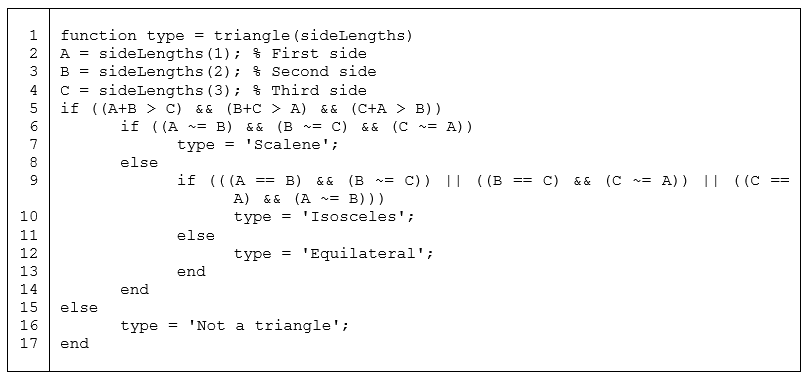
\includegraphics[width=230pt]{gambar/tA2008}
	\caption{\textit{Kode program tA2008}}
	\label{fig:tA2008}
\end{figure}

\subsubsection*{Mengurai Kode Progam ke Format XML}
Penguraian kode program matlab dilakukan dengan menggunakan \textit{library}  MATLAB-PARSER. Kode program yang diinputkan harus sudah dipastikan dapat dijalankan jika di compile. Ketika terdapat kesalahan pada kode program, library  ini akan mengembalikan pesan error. \ref{fig:xml-ta2008} menunjukkan potongan hasil penguraian kode program ke dalam format XML. Potongan kode XML yang terlihat pada \ref{fig:xml-ta2008} menunjukkan hasil penguraian dari kode program pada baris ke 6 sampai baris ke 7.

\begin{figure}
	\centering
	\includegraphics[width=0.9\linewidth]{"gambar/XML tA2008"}
	\caption{Potongan hasil penguraian kode program tA2008 ke dalam format XML}
	\label{fig:xml-ta2008}
\end{figure}

\subsubsection*{Membangkitkan \textit{Graph}}
Salah satu cara untuk membaca dan menulis dokumen XML pada framework .NET dan C\# yaitu dengan menggunakan kelas XMLDocument yang terdapat dalam \textit{namespace System.XML}. Setiap elemen XML yang merupakan struktur kontrol pada program akan menjadi \textit{node} baru di dalam kelas \textit{graph}. Setiap \textit{node} berisi informasi nomor baris dan kolom yang akan digunakan untuk melakukan instrumentasi. Setiap \textit{node} juga dapat memiliki \textit{edge} yang berisi informasi \textit{node} tujuan dan tipe dari garis penghubung itu sendiri. Terdapat tiga macam tipe pada edge yaitu \textit{null}, \textit{true}, dan \textit{false}. \textit{True} dan \textit{false} digunakan jika \textit{node} asal merupakan percabangan.

Hasil \textit{node} yang dibentuk dari kode program tA2008 dapat dilihat pada \ref{fig:hasil-node}. \textit{Node} 1 dibentuk pada awal kode program sebagai inisialisasi. \textit{Node} ditambahkan ketika bertemu dengan perintah yang termasuk ke dalam struktur kontrol seperti IF-ELSE-END, SWITCH-CASE, FOR, dan WHILE. Seperti dapat dilihat pada baris kode ke 5, terdapat perintah IF sehingga dibentuk node baru yaitu \textit{node} 2. 
\begin{figure}
	\centering
	\includegraphics[width=0.9\linewidth]{"gambar/hasil node"}
	\caption{Hasil nodes yang terbentuk dari tA2008}
	\label{fig:hasil-node}
\end{figure}
Representasi objek dari kelas \textit{graph} yang terbentuk dari kode program tA2008 dapat dilihat pada \ref{fig:objectdiagram}. Terbentuk 9 buah \textit{node} dan 11 buah \textit{edge} yang menghubungkan antar \textit{node} tersebut.
\begin{figure}
	\centering
	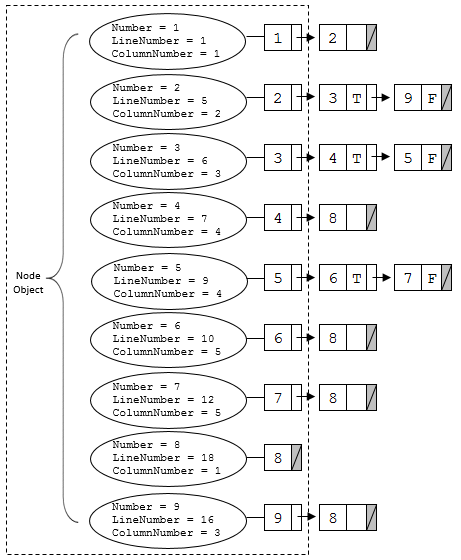
\includegraphics[width=0.9\linewidth]{gambar/ObjectDiagram}
	\caption{Object diagram tA2008}
	\label{fig:objectdiagram}
\end{figure}

\subsubsection*{Membangkitkan Jalur}
Jalur dibentuk dengan cara menelusuri objek graph yang sudah dibentuk sebelumnya. Jika \textit{edge} memiliki tipe \textit{true} atau \textit{false}, maka jalur yang dibangkitkan akan ditambahkan informasi cabang yang dilalui. (T) ketika melalui edge yang memiliki tipe \textit{true}, dan (F)  ketika melalui \textit{edge} yang memiliki tipe \textit{false}. Setiap \textit{edge} memiliki atribut \textit{isVisited} yang digunakan untuk menandai apakah garis penghubung tersebut sudah dilalui atau belum. Jalur yang dibentuk ketika melalui perintah pengulangan seperti FOR dan WHILE akan dibatasi hanya satu kali pengulangan. Berikut merupakan semua kemungkinan jalur yang akan dilalui ketika diberikan suatu inputan yang dapat dijadikan sebagai dasar dalam pembangkitan data uji.
\begin{enumerate}[noitemsep] 
	\item 1 2 (T) 3 (T) 4 8
	\item 1 2 (T) 3 (F) 5 (T) 6 8
	\item 1 2 (T) 3 (F) 5 (F) 7 8
	\item 1 2 (F) 9 8
\end{enumerate}

\subsubsection*{Transformasi ke Dalam Format Bahasa Dot}
Transformasi ke dalam format bahasa dot dilakukan dengan cara menelusuri objek \textit{graph} yang sudah dibangun sebelumnya. Yang didefinisikan dalam bahasa dot adalah \textit{edge} yang terdapat pada \textit{graph} yang dibangun. Seperti yang dapat dilihat pada \ref{fig:dot}, jumlah baris sebanyak jumlah \textit{edge} pada objek graph yang telah didefinisikan sebelumnya.
\begin{figure}
	\centering
	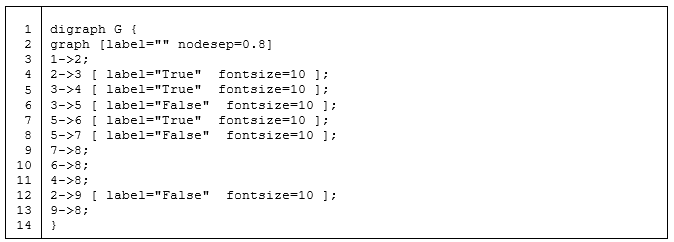
\includegraphics[width=0.9\linewidth]{gambar/dot}
	\caption{Representasi tA2008 dalam bahasa dot}
	\label{fig:dot}
\end{figure}

\subsubsection*{Memvisualisasi \textit{Graph} dalam bentuk CFG}
Setelah file dengan format bahasa dot terbentuk, CFG divisualisasikan dengan menggunakan library Graphviz.Net. Hasil visualisasi bahasa dot kode program tA2008 ke dalam CFG dapat dilihat pada \ref{fig:cfgta2008}.
\begin{figure}
	\centering
	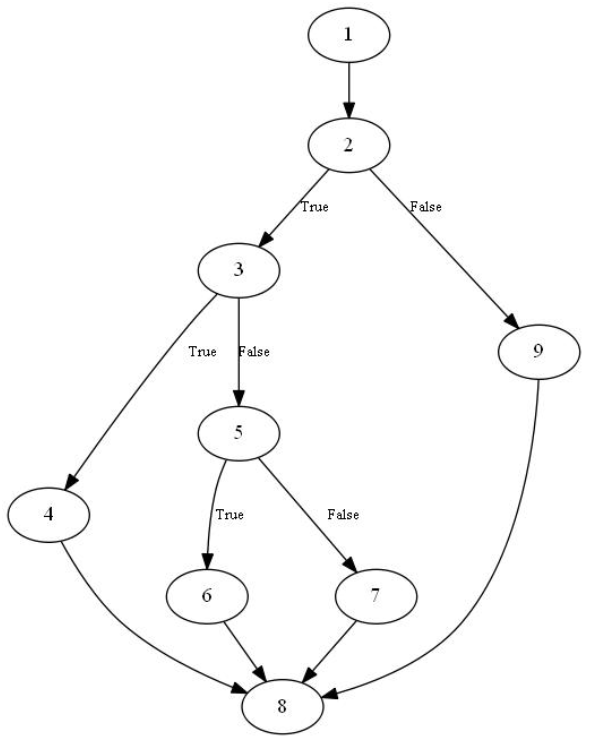
\includegraphics[width=0.9\linewidth]{gambar/cfgtA2008}
	\caption{CFG tA2008}
	\label{fig:cfgta2008}
\end{figure}

\subsubsection*{Menghitung \textit{Cyclometic Complexity}}

\textit{Cyclomatic complexity} merupakan suatu sistem pengukuran yang menunjukkan banyaknya \textit{independent path}. \textit{Cyclomatic Complexity }dihitung dengan cara jumlah \textit{edge} dikurangi dengan jumlah \textit{node}, lalu ditambahkan dengan dua. Berdasarkan graph yang telah terbentuk dari kode program tA2008, dapat dilihat pada \ref{fig:objectdiagram} bahwa jumlah \textit{node} yang terbentuk adalah 9 dan jumlah \textit{edge} yang terbentuk adalah 11. Sehingga hasil perhitungan cyclomatic complexity dapat dilihat pada persamaan dibawah ini.
\[Nodes (N) = 9\]
\[Edges (E) = 11\]
\[V(G) = E - N + 2\]
\[     = 4\]

\subsubsection*{Instrumentasi}
Instrumentasi dilakukan dengan cara menambahkan dulu variabel keluaran bernama traversedPath. Variabel in digunakan untuk menyimpan informasi node mana saja yang dilalui ketika diberikan inputan dengan nilai tertentu. Dan menyimpan informasi pilihan yang dilalui ketika ditemukan cabang yang terdapat pilihan \textit{true} atau \textit{false}.

Hasil kode program yang telah diinstrumentasi dapat dilihat pada Gambar 13. Sebelumnya, kode program tA2008 hanya mengembalikan keluaran satu variabel bernama type yaitu menunjukan jenis dari segitiga ketika diberikan panjang dari ketiga sisi segitiga. Setelah dilakukan instrumentasi, kode program tA2008 akan mengembalikan keluaran dengan variabel tambahan bernama traversedPath.  Sehingga ketika program tersebut dijalankan dengan inputan tertentu akan menghasilkan keluaran nilai traversedPath dan type seperti yang dapat dilihat pada Gambar \ref{fig:instrumentasi}.

Sehingga ketika kode program hasil instrumentasi dijalankan dengan inputan tertentu akan menghasilkan keluaran variabel traversedPath dan type seperti yang dapat dilihat pada Gambar \ref{fig:hasilekseskusi}. Misalkan inputan adalah 3, 4, dan 4 akan menghasilkan isosceles dan dapat diketahui bagaimana cara menghasilkan keluaran tersebut dari traversedPath. 
\begin{figure}
	\centering
	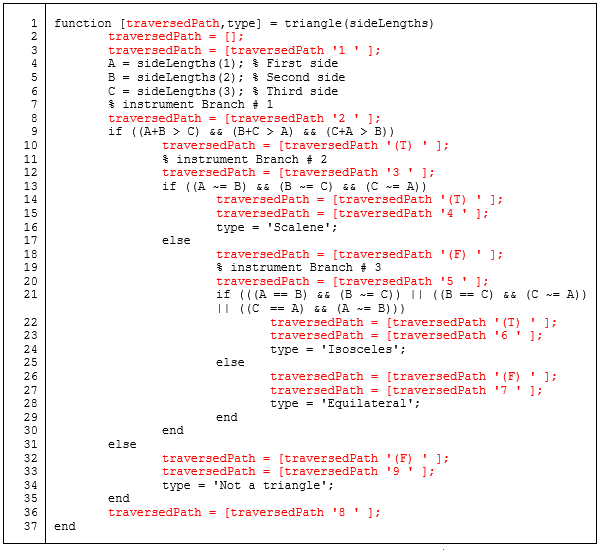
\includegraphics[width=0.9\linewidth]{gambar/instrumentasi}
	\caption{Hasil instrumentasi tA2008}
	\label{fig:instrumentasi}
\end{figure}
\begin{figure}
	\centering
	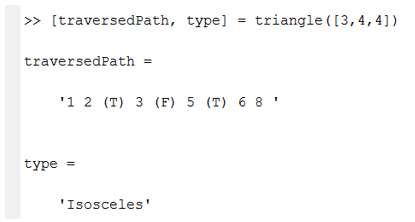
\includegraphics[width=0.7\linewidth]{gambar/hasilekseskusi}
	\caption{Hasil ekseskusi kode program tA2008 yang sudah diinstrumentasi}
	\label{fig:hasilekseskusi}
\end{figure}

\subsubsection*{Implementasi Antarmuka}
Tampilan hasil pembangkitan dapat dilihat pada Gambar \ref{fig:implementasiantarmuka}.

\begin{figure}
	\centering
	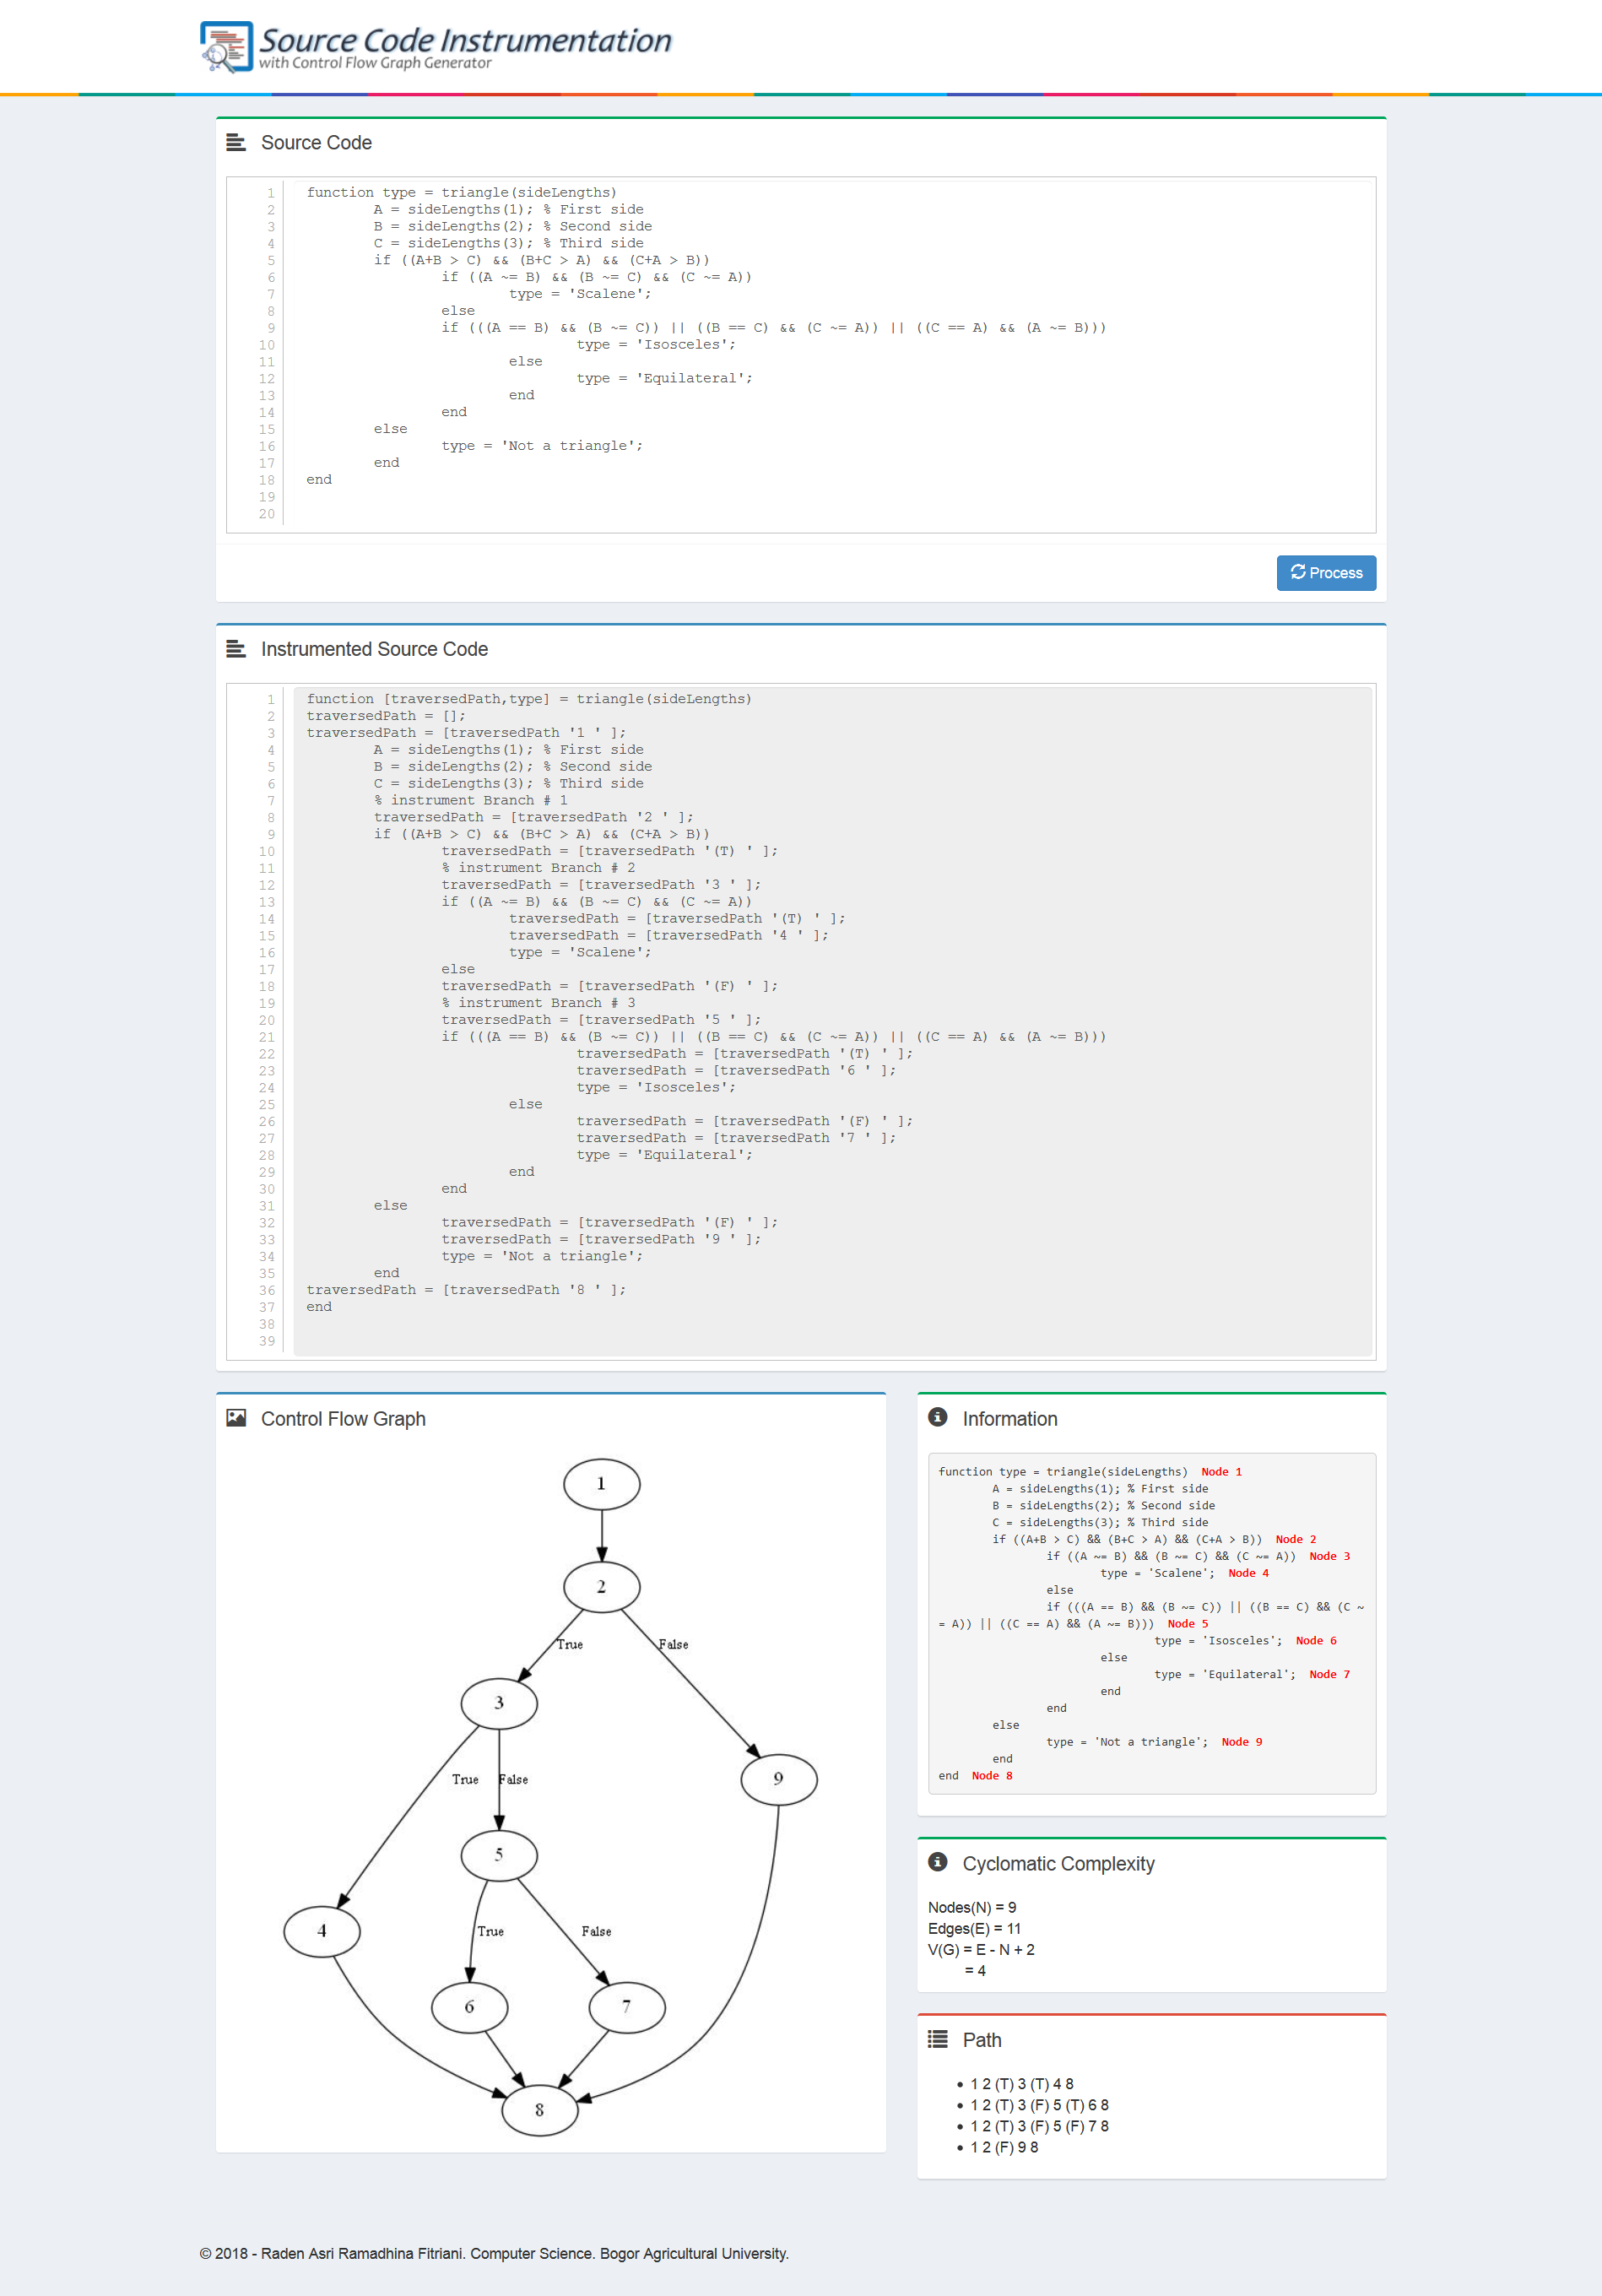
\includegraphics[width=0.9\linewidth]{gambar/implementasiantarmuka}
	\caption{Tampilan hasil pembangkitan}
	\label{fig:implementasiantarmuka}
\end{figure}

\subsection*{Testing}

Tahapan ini adalah melakukan evaluasi dari tahapan implementasi. Evaluasi dilakukan dengan membandingkan hasil yang dikeluarkan oleh sistem dengan pembangkitan secara manual dari segi waktu eksekusi. Penguji terdiri dari dua orang yang berprofesi sebagai pengembang sistem. 

Hasil jalur yang dibentuk dan nilai \textit{cyclomatic complexity} dari program uji dapat dilihat pada Tabel 2. Hasil perbandingan waktu yang dibutuhkan untuk melakukan pembangkitan secara manual dan oleh aplikasi dapat dilihat pada Tabel 3.
\begin{table}
	\centering
	\caption{Hasil jalur dan \textit{cyclomatic complexity} dari program uji}
	\label{tab:tabeljalur}
	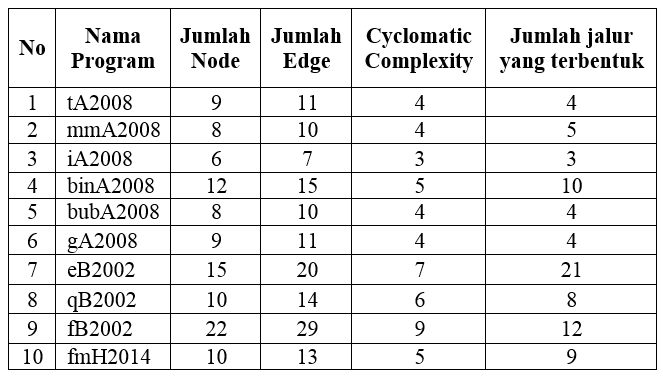
\includegraphics[width=0.9\linewidth]{gambar/tabeljalur}
\end{table}

Jumlah jalur yang terbentuk bisa lebih besar dari cyclomatic complexity karena jumlah jalur yang tebentuk adalah dari semua kemungkinan. Sedangkan jumlah cyclomatic complexity menunjukkan independent path yaitu jalur yang setidaknya ada 1 jalur baru yang dilalui.    

\begin{table}
	\centering
	\caption{Perbandingan eksekusi secara menual dan oleh aplikasi}
	\label{fig:tabelperbandingan}
	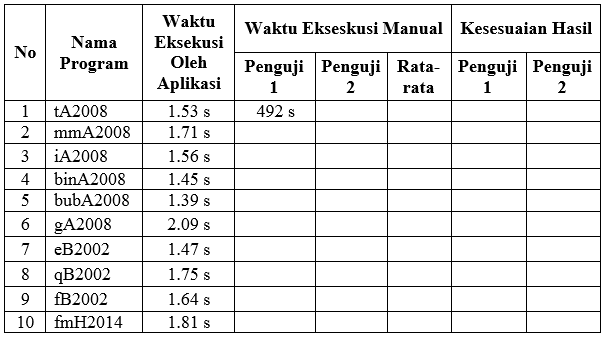
\includegraphics[width=0.9\linewidth]{gambar/tabelperbandingan}
\end{table}


